\documentclass[11pt]{beamer}
\usetheme{Copenhagen}
\usepackage[utf8]{inputenc}
\usepackage[spanish]{babel}
\usepackage{amsmath}
\usepackage{amsfonts}
\usepackage{amssymb}
\usepackage{graphicx}
\author{Elena María Gómez Ríos y Jose Luis Martínez Ortiz}
\title{Comparativa entre Systemd e init}
%\setbeamercovered{transparent} 
%\setbeamertemplate{navigation symbols}{} 
%\logo{} 
%\institute{} 
%\date{} 
%\subject{} 
\begin{document}

\begin{frame}
\titlepage
\end{frame}

\begin{frame}
\begin{enumerate}
\item ¿Qué es Init?
\item System V init
\item ¿Qué es Systemd?
\item Estructura
\item Demonios
\item Ventajas
\item Desventajas
\item Controversia generada
\item Conclusiones
\end{enumerate}
\end{frame}


\begin{frame}{¿Qué es Init?} % 1
Es el proceso encargado del inicio de sistemas \texttt{Linux}.\\
\vspace{1cm}
El proceso init se caracteriza por su simpleza y facilidad de uso. El funcionamiento de init consiste en ir iniciando los procesos listados en un archivo de configuración, es decir, inicia el primer proceso del listado y cuando éste se ha iniciado inicia el siguiente y así sucesivamente.
\end{frame}
% -----------------------------------------------------
\begin{frame}{System V init} % 2
System V es una versión mejorada del init original, que consiste en un sistema de llamadas por niveles de prioridad para la ejecución de los procesos del sistema.


\begin{figure}[H] %con el [H] le obligamos a situar aquí la figura
\centering
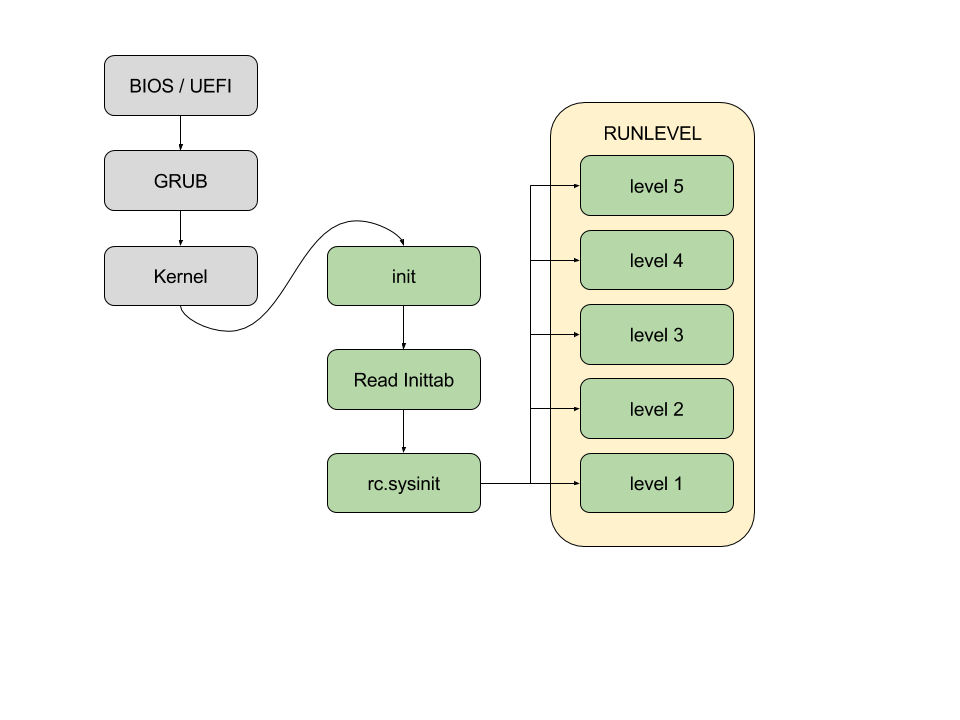
\includegraphics[scale=0.3]{../imagenes/System_V.png} 
\label{fig:System_V}
\end{figure}


\end{frame}

% -----------------------------------------------------
\begin{frame}{¿Qué es Systemd?} % 3
\texttt{Systemd} fue desarrollado por Lennart Poettering y Kay Sievers, ambos empleados de Red Hat.

\vspace{0.5cm}

Es una suite o conjunto de herramientas diseñadas para facilitar y mejorar el arranque del sistema operativo. Específicamente es un conjunto de demonios de \textit{Linux}.

\vspace{0.5cm}

Systemd no solo ha sustituido al proceso init, sino a toda la gestión que era necesaria para el correcto funcionamiento del inicio del sistema.

\end{frame}

% -----------------------------------------------------
\begin{frame}{Estructura} % 4

\begin{figure}[H] %con el [H] le obligamos a situar aquí la figura
\centering
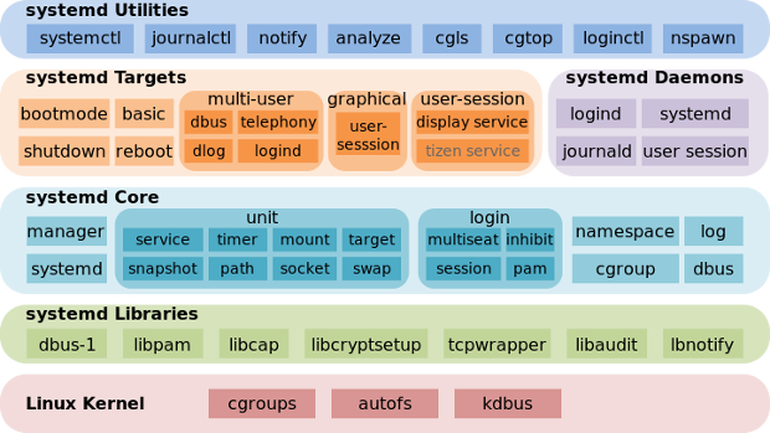
\includegraphics[scale=0.42]{../imagenes/systemd_components.png} 
 \label{fig:systemd_components}
\end{figure}

\end{frame}

% -----------------------------------------------------
\begin{frame}{Demonios} % 5
Los principales demonios de systemd son:
\vspace{0.5cm}
\begin{itemize}
\item \textbf{Demonio journald.} Gestiona los mensajes del sistema (logs).
\item \textbf{Demonio logind.} Es el encargado de administrar los inicios de sesión del sistema.
\item \textbf{Demonio user session.} Su función es permitir o bloquear los inicios de sesión de usuario dependiendo del estado del sistema.
\end{itemize}
\end{frame}

% -----------------------------------------------------
\begin{frame}{Ventajas systemd frente a init} % 6

\begin{itemize}
\item Mejor gestión de las dependencias.
\item Utiliza la paralelización para el inicio de los procesos.
\item Su configuración es compatible con las versiones de init.
\item Tiene mayor velocidad en el arranque del sistema.
\item Optimiza el uso de recursos utilizando \texttt{cgrups}.
\end{itemize}

\end{frame}

% -----------------------------------------------------

\begin{frame}{Desventajas systemd frente a init} % 7

\begin{itemize}
\item Tiene una implementación fuertemente ligada.
\item Requiere de un conjunto de paquetes extra, como son: ACL, PAM, DBus y polkit.
\item Genera mayor sobrecarga al sistema.
\item No sigue la filosofía clásica de ``Unix''.
\end{itemize}

\end{frame}

% -----------------------------------------------------
\begin{frame}{Controversia generada} % 8

Se puede encontrar un gran número de desarrolladores completamente en contra de systemd como sistema de arranque.

\vspace{0.5cm}

Utiliza el mismo enfoque que los sistemas operativos modernos, de abstraer al usuario de la configuración del sistema creando una ``caja negra''. No se accede directamente a los archivos de configuración sino que se hace a través del framework.

\end{frame}

% -----------------------------------------------------
\begin{frame}{Conclusiones} % 9

Podemos decir que en \textbf{ordenadores personales} es una ventaja utilizar \textbf{systemd} en vez de init, ya que para un uso normal del sistema es preferible un inicio más rápido y una mayor abstracción de la administración del sistema teniéndolo todo unificado, como ya hacen Windows o Mac.

\vspace{0.5cm}

Sin embargo en el mundo de los \textbf{servidores} donde es tan importante la sobrecarga del sistema producida por el propio sistema y sus componentes, es preferible un sistema de arranque más lento, como \textbf{init}, pero con mucha menos sobrecarga. Además systemd dificulta la administración del servidor por su compleja implementación.

\end{frame}


\end{document}